\documentclass[12pt,onecolumn,a4paper]{report}
\usepackage{epsfig,graphicx,subfigure,amsthm,amsmath}
\usepackage{color,xcolor}     
\usepackage{xepersian}
\usepackage{graphicx}
\usepackage{sectsty}
\settextfont[]{B-NAZANIN.TTF}
\setlatintextfont[Scale=1]{Times New Roman}
\usepackage{geometry}
 \geometry{
 a4paper,
 total={170mm,257mm},
 left=20mm,
 top=20mm,
 }

\begin{document}
%\text{گزارش پروژه کارشناسی}
\title{
\includegraphics[width=5cm, height= 5cm]{3.jpg}\\\Large{دانشکده فیزیک}\\{\LARGE{گزارش پروژه کارشناسی}}\\{\\{\Huge{عنوان پروژه:}\\\Huge{شبیه سازی برهمکنش غشا لیپیدی و نانو ذرات \\با استفاده از نرم افزار \lr{VCM} }}} }
\author{\LARGE{استاد پروژه : دکتر محمدرضا اجتهادی}\\\LARGE{یگانه بهاری - فهیمه فخری}}
\date{\LARGE{\today}}
\maketitle
\tableofcontents

\section{\LARGE{مقدمه} }
\large{غشای سلولی شامل دو لایه فسفولیپیدی همراه با پروتئین است. مولکول فسفولیپید از اتصال یک سر شامل گروه فسفات
به یک یا دو زنجیره هیدروکربنی تشکیل شده است
مولکول های چربی با قرار دادن زنجیره هیدروکربنیشان
رودرروی یکدیگر، تشکیل یک غشای دو لایه میدهند.سر شامل گروه فسفات دارای خاصیت آبدوستی و دم شامل زنجیره هیدروکربنی دارای خاصیت
آبگریزی است. با تجمع پروتئینهای شامل ساختار
آب گریز بر یک طرف غشا، دم آبگریز این پروتئینها وارد غشای لیپیدی (یعنی ناحیه
شامل زنجیره های هیدروکربنی) میشود ومیتواند منجر به ایجاد
انحنا در غشا شود.ورود و خروج بسیاری از باکتری ها به صورت نانوذره به این صورت رخ میدهد.\\
تمرکز این پروژه روی شبیه سازی برهمکنش غشا با آن دسته از نانوذراتی است که بدون استفاده از عوامل خارجی و فقط به کمک جاذبه میان غشا و ذرات باعث تغییر شکل غشا میشوند.
هدف اصلی مشاهده دینامیک سیستم برهمکنش غشا و نانوذرات است که به کمک نرم افزار\lr{VCM}  انجام میشود.
ما در طول انجام این پروژه تجربیاتی کسب کرده ایم و کارهایی انجام داده ایم که در طول این گزارش به آنها اشاره خواهیم کرد. در نهایت با مقادیری که برای پارامتر های مربوطه پیدا کرده و به دست آورده بودیم موفق به مشاهده حرکت نانوذرات بر روی غشا و نزدیک شدن دو نانوذره به یکدیگر شدیم.
در آخر تشکر بسیار از دکتر اجتهادی و آقای علی فرنودی داریم که صبورانه در این پروژه ما را همراهی و راهنمایی کردند و آموخته های بسیاری را به ما ارزانی داشتند.\\
*لینک تمامی ارجاعاتی که در گزارش حرفشان را زده ایم در قسمت مراجع قرار داده ایم.}



\section{\LARGE{نصب و شروع کار با نرم افزار}}
\large{در ابتدا این را بدانید که بهتر است نرم افزار را روی سیستم عامل لینوکس نصب کنید. ما از بین توزیع های لینوکس اوبونتو را انتخاب کردیم. اگر سیستم عامل ویندوز دارید میتوانید به راحتی منابع فارسی و انگلیسی در اینترنت برای راهنمایی نصب اوبونتو بر روی سیستم عامل ویندوز پیدا کنید. اما در مراحل نصب نرم \lr{VCM} نتوانستیم \lr{Opencl} را بر روی اوبونتو 20 نصب کنیم. در حالی که نصب \lr{Opencl} بر روی اوبونتو 18 و 16 ممکن بود. و یکی از ما با اوبونتو 18 و دیگری با اوبونتو 16 شروع به کار کردیم. نسخه \lr{Opencl} ای که نصب کردیم را روی گیت هاب به اشتراک گذاشته ایم. به هنگام به کار گرفتن برهمکنش در استفاده از نرم افزار \lr{VCM} در اوبونتو 18 این نسخه \lr{Opencl} کار نمیکند. \\
برای مراحل بعدی نرم افزار میتوانید از راهنمای نصب سایت نرم افزار استفاده کنید.\\
برای نمایش خروجی گرفته شده از نرم افزار \lr{VCM} هم از نرم افزار \lr{vmd} استفاده کردیم که به راحتی و به کمک راهنمایی های موجود در اینترنت میتوان این نرم افزار را نصب کرد و ما به مشکلی برنخوردیم.\\
پس از نصب نرم افزار همانطور که در راهنمای نصب هم گفته شده است با وارد کردن دستور  \lr{./VCM -h} در ترمینالی که در پوشه  \lr{bin} نرم افزار باز میکنید، همه دستورات را برای کار با نرم افزار به همین آدرس میدادیم، میتوانید راهنمایی اولیه درباره ی کار با نرم افزار را بگیرید.\\
ما برای کار با نرم افزار از دستور هایی که الان شرح میدهیم استفاده کردیم. اول از هرچیزی باید به کمک نرم افزار یک  \lr{configuration file} بسازید که نرم افزار این فایل را در همان جایی که ترمینال را باز کرده اید یعنی در پوشه  \lr{bin} و در قالب فایل تکست ذخیره میکند. این فایل درواقع حاوی همه مشخضاتی است که برای شبیه سازی خود در نظر دارید. میتوان از دو طریق این فایل را به وجود آورد. یکی از راه ها از طریق دستور  \lr{./VCM -g 0} می باشد که در این صورت همانطور که در تصویر 1 مشاهده میکنید تنها نام فایل را انتخاب میکنید و تصمیم میگیرید که توضیحات هر متغیری در فایل نوشته شده باشد یا خیر. که برای اولین تجربه کار با نرم افزار بهتر است کامنت ها را ببینید و توضیحات در کامنت ها به حد کفایت است. پس از ساخت فایل میتوانید فایل را باز کنید و مقادیر متغیر هایی که میخواهید را وارد کنید.\\
\begin{center}
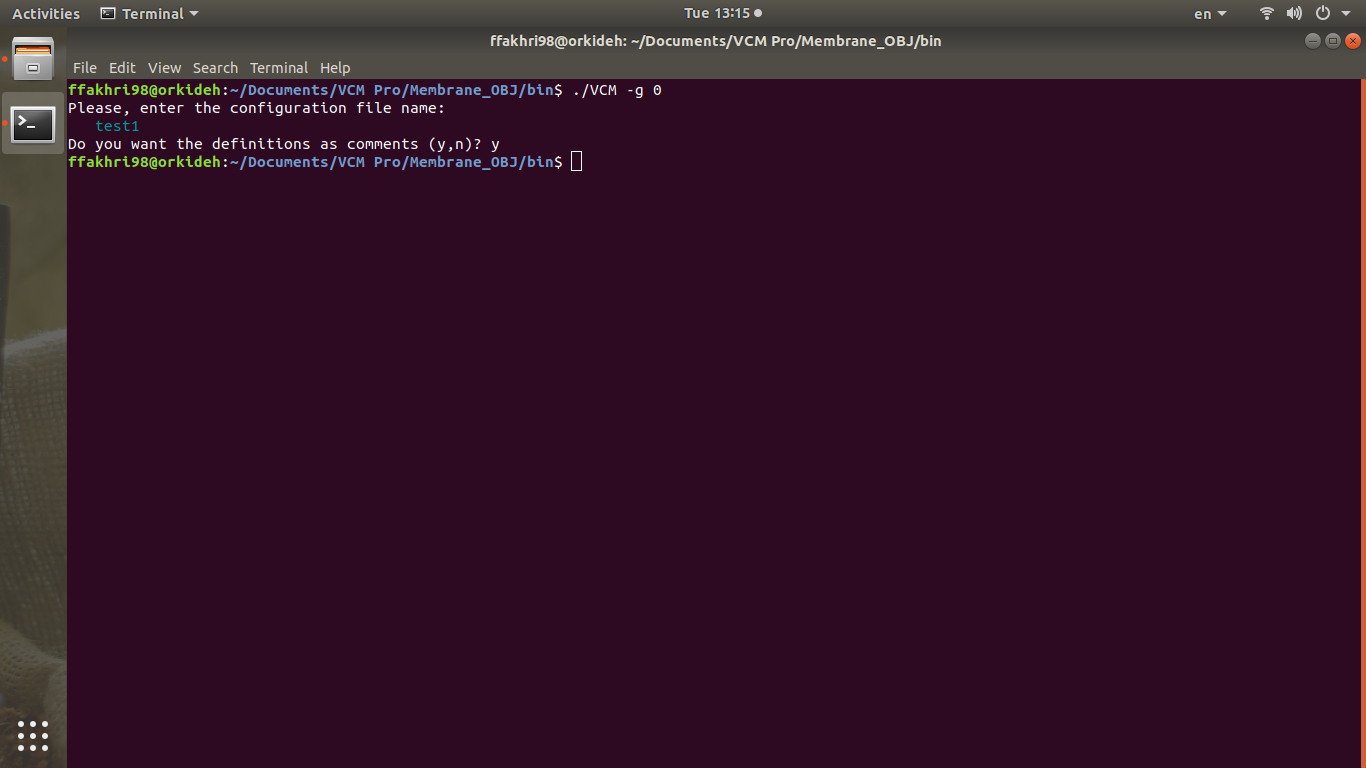
\includegraphics[width=16cm, height=9cm]{01.png}
\caption{تصویر 1}
\end{center}\\
*فایل را به دقت مطالعه کنید.\\
راه دیگر ساختن این فایل از طریق وارد کردن دستور \lr{./VCM -g 1} می باشد که در این صورت متغیر هایی را در همین حین یعنی در ترمینال وارد میکنید. در تصویر 2 مشاهده میکنید.\\
\begin{center}
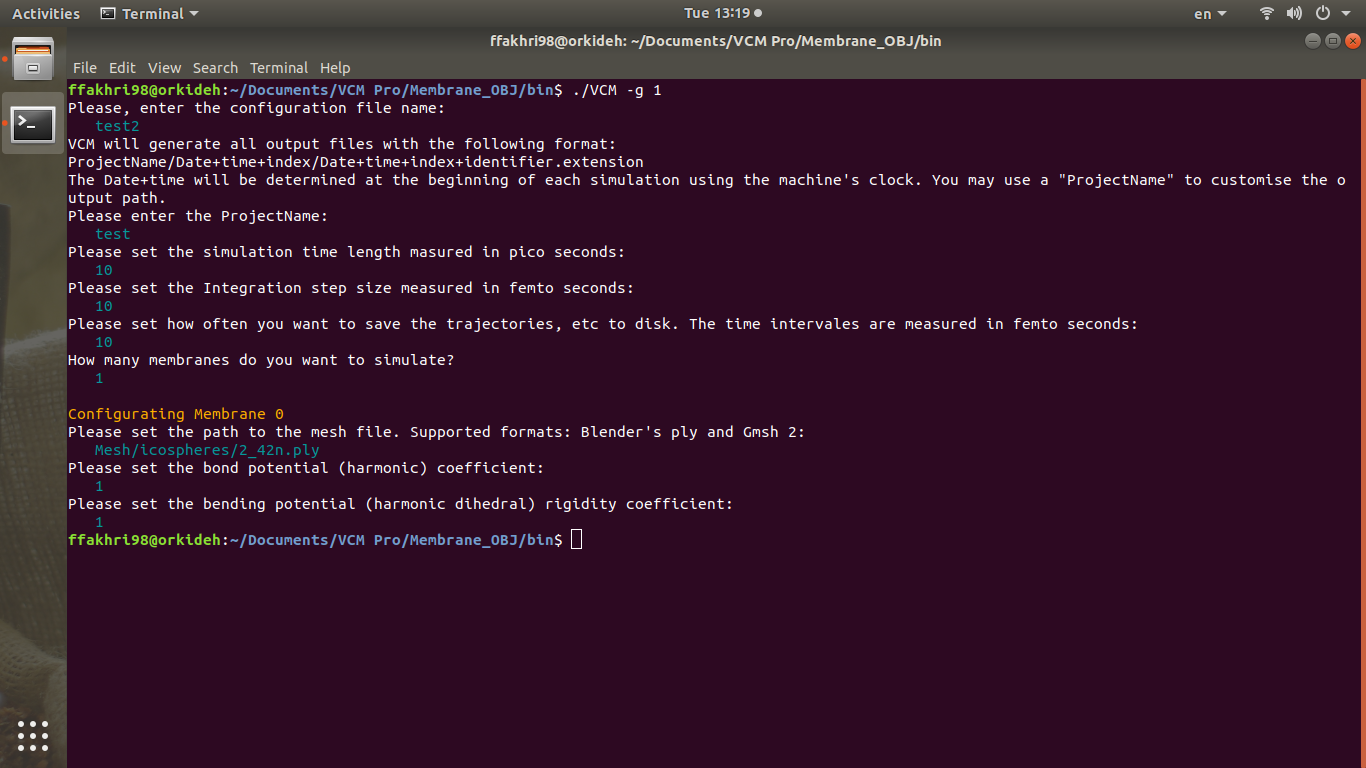
\includegraphics[width=16cm, height=9cm]{02.png}
\caption{تصویر 2}
\end{center}\\
و مانند روش قبل در اینجا هم پس از ساخته شدن فایل میتوانید بروید فایل را باز کنید و تغییراتی در متغیر های ایجاد کنید و یا متغیر های تازه ای را روشن کرده و وارد داستان کنید.\\
*توجه شما را به قسمتی در تصویر 2 که  \lr{mesh file} نوشته شده جلب میکنم. ما از مش های آماده ای که در همین آدرس وارد شده در تصویر 2 مشاهده میکنید وجود داشتند استفاده کردیم. عدد بزرگتری که در اسم فایل مش وجود دارد برابر با تعداد ذرات آن مش است. در صورتی که در اسم مش  \lr{n} وجود داشته باشد، آن غشا کاملا به شکل کره خواهد بود و در غیر اینصورت غشا نقاط نقص خواهد داشت و کاملا کروی نخواهد بود.\\
\begin{center}
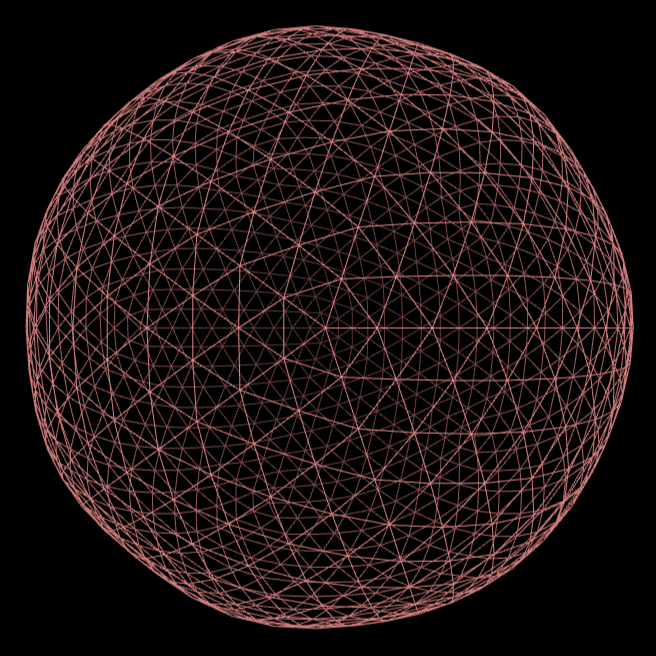
\includegraphics[width=9cm, height=9cm]{03.png}\\
\caption{تصویر 3 : یک مش کروی}
\end{center}\\

\begin{center}
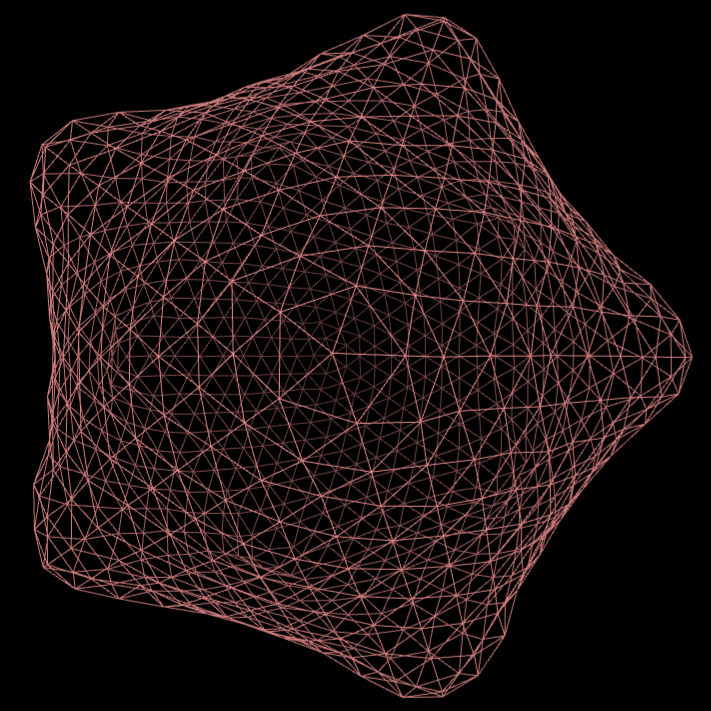
\includegraphics[width=9cm, height=9cm]{04.png}\\
\caption{تصویر 4 : یک مش حاوی نقاط نقص}
\end{center}\\
حال برای اجرای \lr{configuration file} از دستور \lr{./VCM -c} استفاده کردیم به این نحو که اسم  \lr{configuration file} را هم در ادامه دستور مینوشتیم مطابق تصویر 5 و 6 و 7.\\
\begin{center}
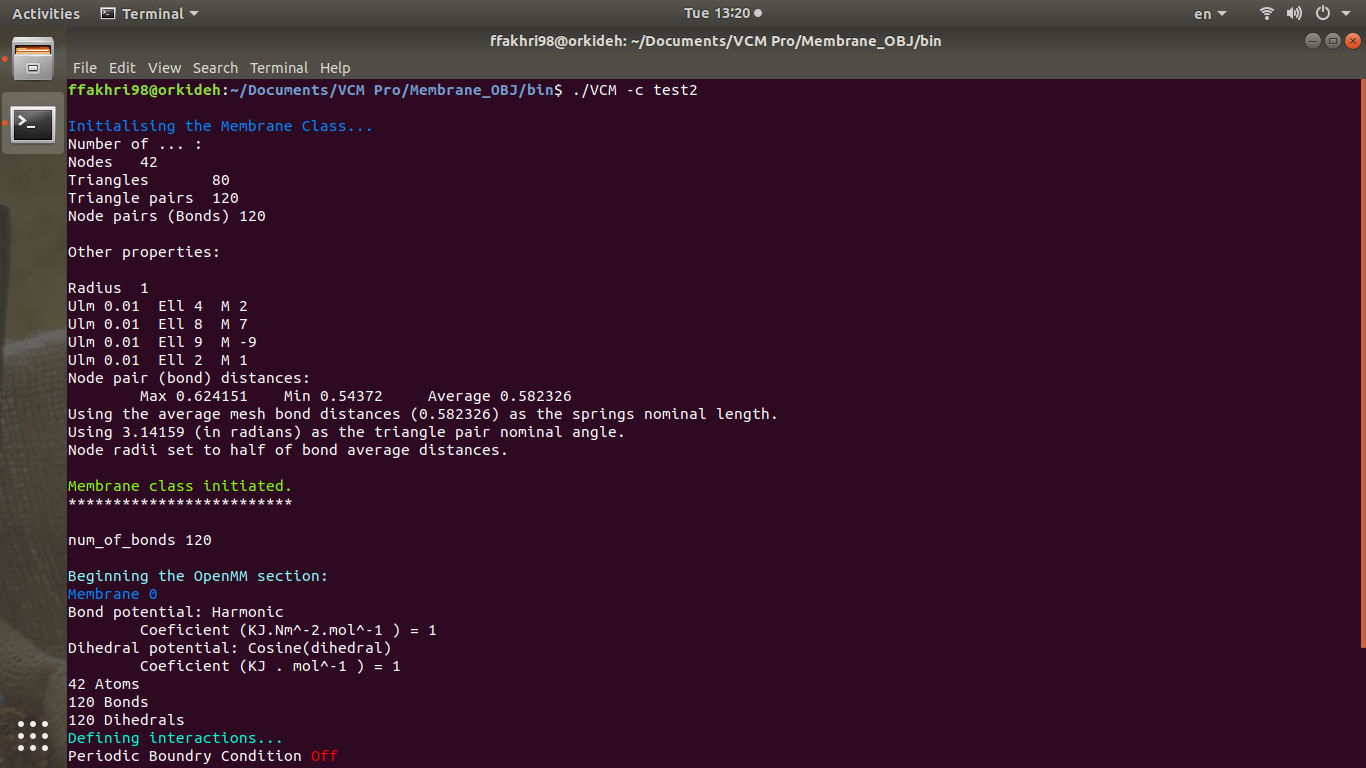
\includegraphics[width=16cm, height=9cm]{05.png}\\
\caption{تصویر 5}
\end{center}\\
\begin{center}
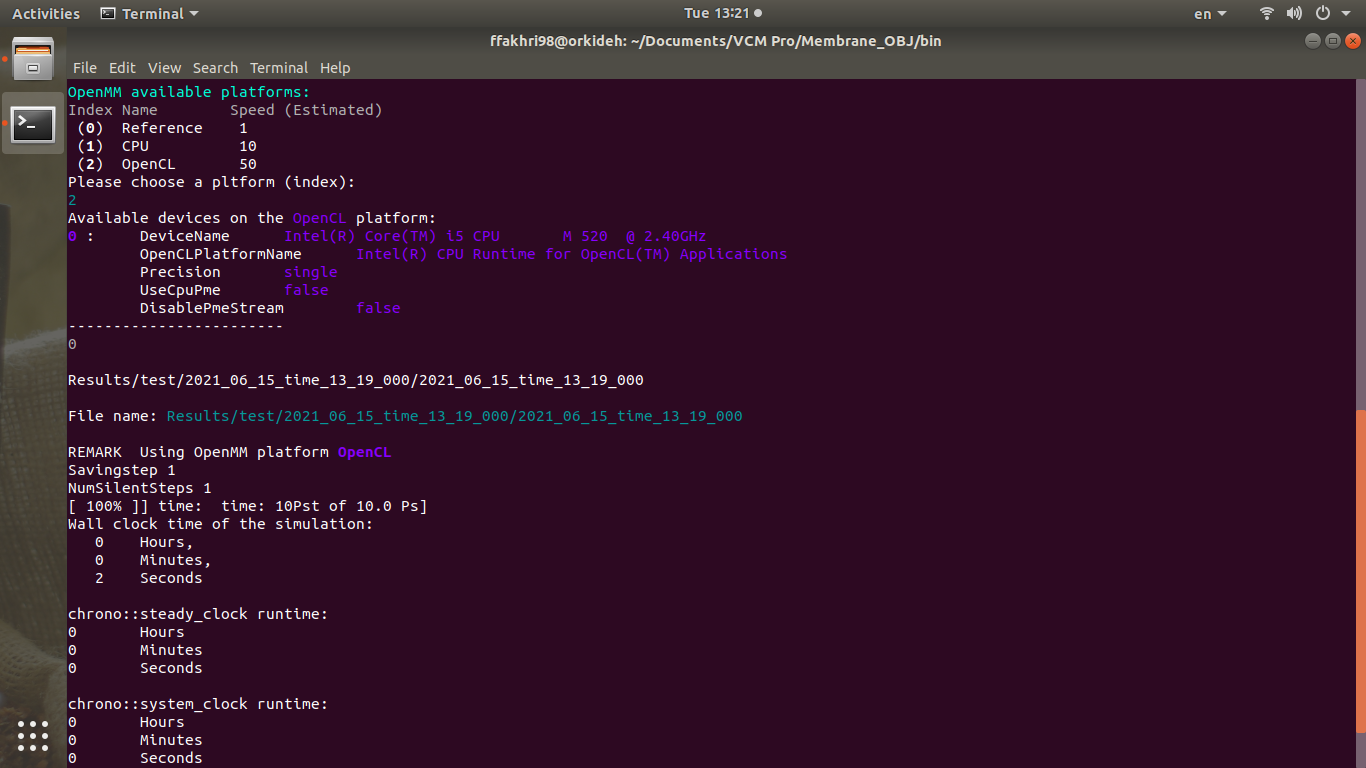
\includegraphics[width=16cm, height=9cm]{06.png}\\
\caption{تصویر 6}
\end{center}\\
\begin{center}
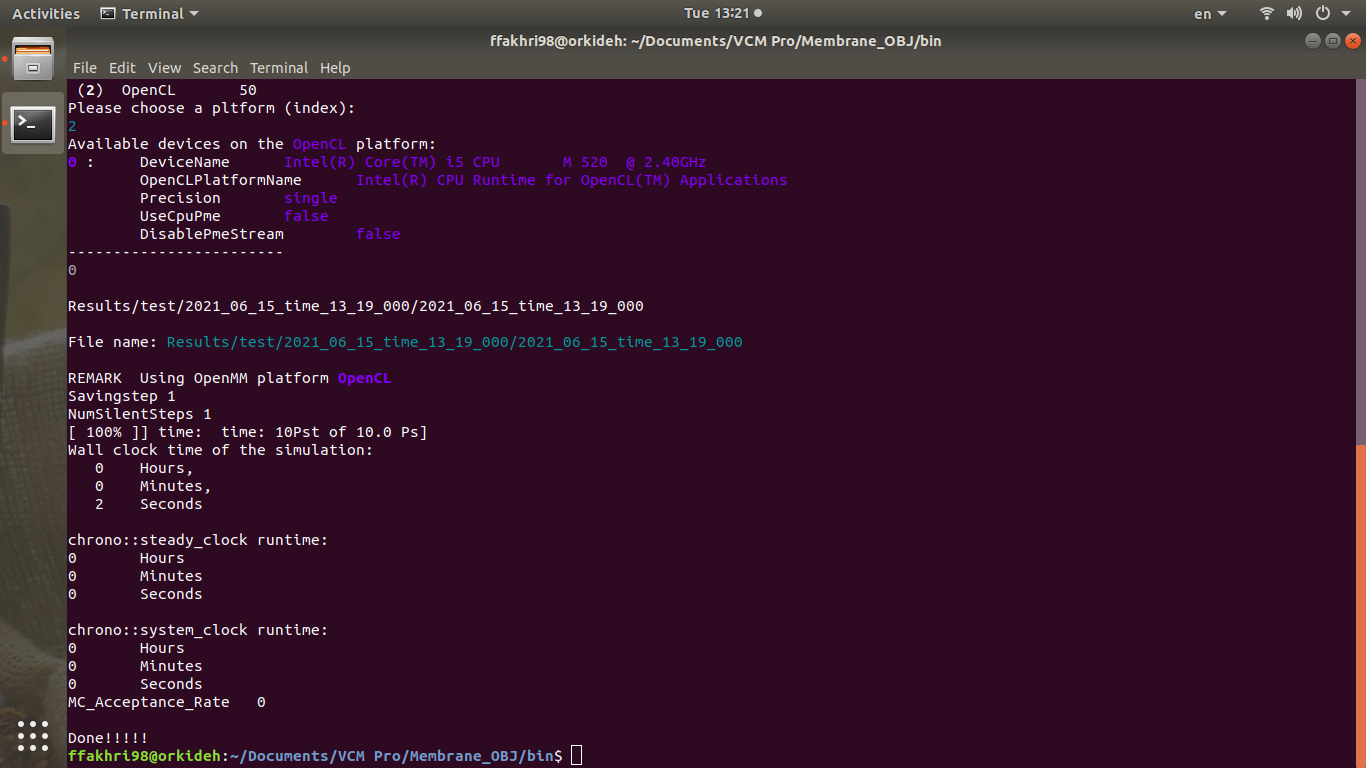
\includegraphics[width=16cm, height=9cm]{07.png}\\
\caption{تصویر 7}
\end{center}\\
همانطور که در تصویر 6 مشاهده میکنید در قسمتی از اجرای این دستور از ما میپرسد که از چه پلتفرمی استفاده کند و وجود \lr{Opencl} بین گزینه های موجود نشاندهنده این است که نصب شده است.\\
اطلاعات خوبی حین اجرای این دستور داده می شود. مثلا همانطور که در تصویر 5 مشاهده میکنید اطلاعاتی درباره ی فاصله ذرات غشا نوشته شده است که به کار می آید.
همانطور که در تصویر 6 مشاهده میکنید آدرس فایل های مربوطه به این اجرا نوشته شده است که ما با وارد کردن فایل های \lr{pdb} و \lr{psf}
در نرم افزار \lr{vmd} نتیجه را مشاهده میکردیم.
}




\section{\LARGE{طرح مساله}}
در مساله شبیه سازی غشا سلولی به به وسیله نرم افزار ابتدا باید تمام واحد های مورد نظر را به واحد های مورد قبول نرم افزار تبدیل کنیم. در قسمت تبدیل واحد درباره واحد های مورد قبول نرم افزار صحبت کرده ایم. از نظر فیزیکی مدلسازی غشا به این صورت انجام میشود که غشا از یک سری فنر های متصل  بهم تشکیل شده است که دارای سختی فنر و سختی خمشی هستند که کل سیستم در یک حمام گرمای قرار دارد .برای شبیه سازی باید معدله نیروی وارد به این فنر ها را حل کنیم تا بتوانیم دینامیک سیستم را پیش بینی کنیم.\\

\lr{VCM} یک بسته نرم افزاری برای انجام شبیه سازی های دینامیک مولکولی است که قادر است
با مدلسازی درشتدانه اجزای مختلف سلول، خواص مکانیکی اجزای سلول را بررسی کند.
% \lr{VCM}ای در دستگاه واحدهای کاهیده صورت میگیرد، 
از آنجا که مدلسازی در \lr{VCM} در دستگاه واحد های کاهیده صورت میگیرد در هر مساله با ترجمه واحد های مورد نظر به واحد های قابل قبول نرم افزار میتوان طیف وسیعی از فرایند های بیولوژیکی را شبیه سازی کرد.\\
در این پروژه تلاش کردیم تا با جستجو و یافتن پارامتر های واقعی غشا و نانوذرات همانند سختی خمش و سختی فنر  تبدیل آن ها به واحد های نرم افزار یک شبیه سازی واقعی انجام دهیم.




\section{\LARGE{روش شبیه سازی}}
پس از آشنایی های اولیه با طرز کار نرم افزار دیگه باید سراغ دیتا گرفتن از نرم افزار میرفتیم و برای شروع اینکار و دست به کار شدن با نرم افزار پارامتر های سختی فنر و سختی خمشی را روشن کردیم و به ازای شعاع های مختلف تلاش کردیم مقادیری را پیدا کنیم که غشا با داشتن آن مقادیر برای دو پارامتر گفته شده حالت پایداری داشته باشد. یعنی ناگهان متلاشی نشود و حالت خودش را خوب حفظ کند. برای تغییر شعاع باید پارامتر \lr{scale} را تغییر میدادیم. با دیتا گرفتن  و مشاهده غشا و راهنمایی گرفتن از آقای فرنودی بالاخره مقادیر مناسب برای داشتن غشا پایدار را پیدا کردیم و نمودار هایی را برای تغییرات شعاع این ممبرین ها رسم کردیم. برای رسم این نمودار ها از فایل \lr{pdb} استفاده کردیم و یک کد پایتون هست که آنرا در گیت هاب قرار داده ایم. کافیست تکه ساده ای به این کد اضافه کنید تا بتوانید با دادن فایل \lr{pdb} به کد نمودارات تغییر شعاع را ببینید. نمودار های 1 و 2 و 3 با مشخصاتی که روی آنها نوشته شده حاصل کار ما در این قسمت بوده است. همانطور که مشاهده میکنید برای یکی از غشا ها سرعت اولیه هم در نظر گرفته بوده ایم.\\.
\begin{center}
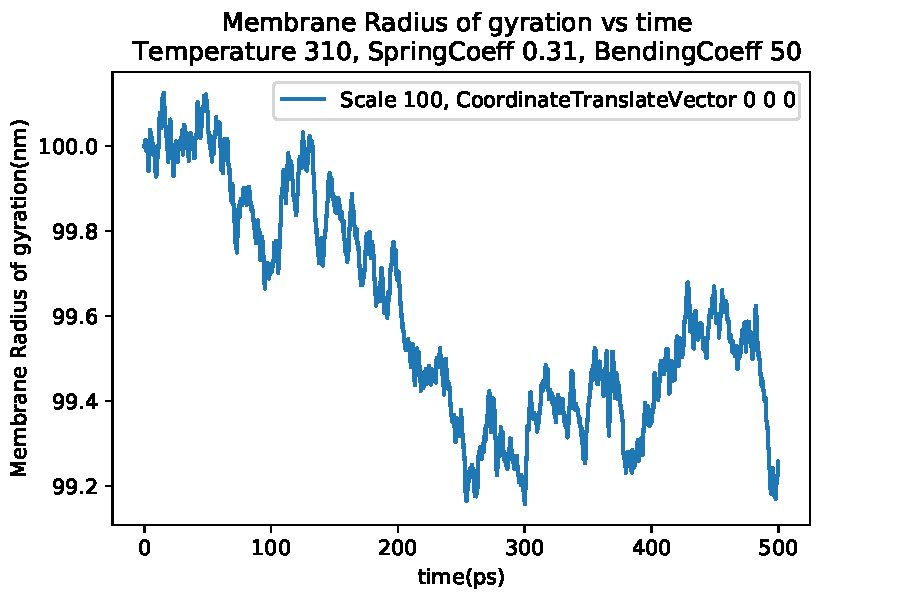
\includegraphics[width=16cm, height=9cm]{1.pdf}\\
\caption{نمودار 1}
\end{center}\\
\begin{center}
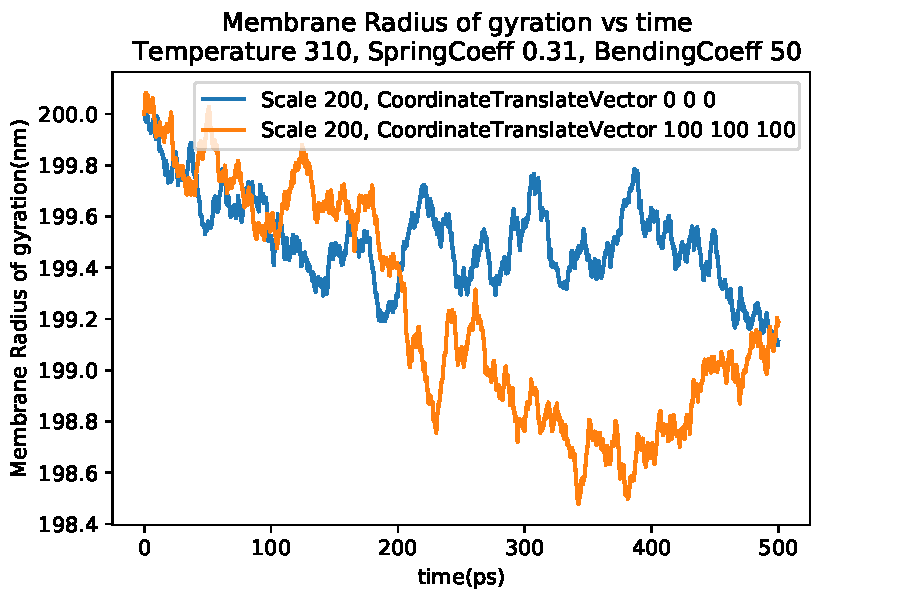
\includegraphics[width=16cm, height=9cm]{2.pdf}\\
\caption{نمودار 2}
\end{center}\\
\begin{center}
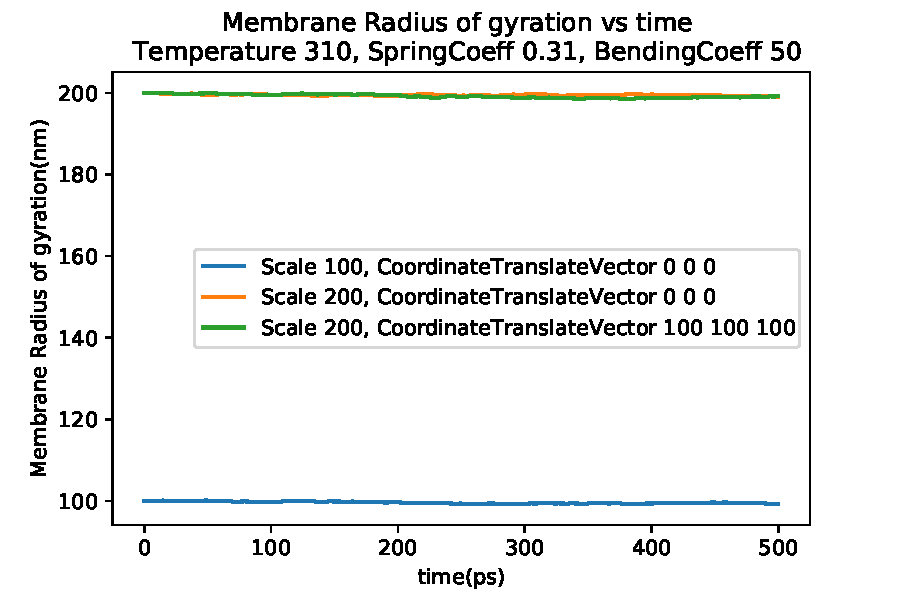
\includegraphics[width=16cm, height=9cm]{3.pdf}\\
\caption{نمودار 3}
\end{center}\\
پس از این مقدمات
برای حل این مساله ابتدا تلاش کردیم تا به وسیله جستجو و مطالعه واحد های واقعی مورد نظر را بیابیم. نرم افزار\lr{VCM} غشای لیپیدی را به وسیله مش بندی مثلثی شبیه سازی میکند به این صورت که بین هر دو نقطه از شبکه یک فنر هارمونیک وجود داردو بین هر دو فنر همسایه نیز پتانسیل خمشی اعمال میشود. مجموع این دو پتانسیل خواص کشسان غشا را به وجود می آورد.
در شبیه سازی به وسیله روش دینامیک مولکولی باید معادلات حاکم بر ذرات تشکیل دهنده سیستم را حل کنیم. یکی از الگوریتم های معمول در این نوع شبیه سازی الگوریتم ورله سرعتی است که در سیستم های زیستی  در صورت استفاده از این الگوریتم باید برای سیستم ترموسات تعریف شود تا دما ثابت بماند. اما ترموستات اگرچه دما را ثابت میکند اما نمی تواند حرکات ذرات بر اثر افت و خیز را شبیه سازی کند. یک راه حل مناسب استفاده از دینامیک لانژون است به این ترتیب که با حل این معادله میتوان سیستم غوطه ور در حمام گرمایی را شبیه سازی کرد.\\
در ابتدا باید محیط متناسب برای غشا را با توجه به انچه در آزمایشگاه مشاهده کردیم اعم از دمای محیط و روش حل معادلات حاکم بر سیستم را  در نرم افزار مشخص کنیم.پس از آن به سراغ تنظیم پارامتر های غشا میرویم.\\
غشاهای زیستی به دلیل پخش سطحی مولکولهای
چربی سازنده شان، مانند مایع دوبعدی عمل میکنند. این خاصیت با تغییر اتصال نقاط شبکه
در طی شبیه سازی بازنمایی می شود. طی این فرآیند، انرژی مکانیکی غشا از طریق انتخاب های
مونت-کارلو برای یافتن بهترین پیکربندی شبکه کمینه میشود.
در نتیجه برای شبیه سازی غشا لیپیدی که فیزیک آن شبیه غشای لیپیدی واقعی دیده شده در آزمایشگاه باشد باید پارامتر های سایز غشا  و سختی خمشی و سختی فنر را بدست آوریم .برای بدست آوردن واحد ها به مقالات مختلفی که در انتهای گزارش به آن ها ارجاع داده شده رجوع کردیم و با استفاده از شهود خود به عنوان فیزیک پیشه واحد ها را بدست آوردیم.\\
برای شبیه سازی نانوذارت باید ابعاد آن ها را در نظر بگیریم و با توجه به سایز غشا آن ها را تنظیم کنیم.این ذرات انعطاف پذیری بسیار کمتری از غشا دارند و نوعی جسم صلب به حساب می آیند و تنها میتوانند حرکت انتقالی و دورانی حول مرکز جرم خود انجام دهند. در این پروژه این نانوذارت را مشابه با غشا شبیه سازی کرده اما سختی فنر و سختی خمشی آن ها زا به گونه ای تنظیم کرده که به صورت جسم صلب باشند. برای جلوگیری از فرو رفتن نانوذرات در یک دیگر بینشان یک پتانسیل تعریف کرده ایم. \\
یکی از چالش های مهم این پروژه تنظیم برهمکنش میان غشا و نانوذرات و بررسی دینامیک سیستم است. برای این برهمکنش از پتانسیل لنارد جونز استفاده کرده ایم. این پتانسیل برای برهمکنش های کوتاه برد میان غشا و نانو ذرات مناسب است.




\section{\LARGE{تبدیل واحد}}

پیش از هرچیزی همانطور که در قسمت قبل قولش را داده ایم باید که بگوییم واحد پارامتر هایی که ما با آن ها دست به یقه شدیم در نرم افزار چه هست.  واحد انرژی کیلوژول بر مول، واحد جرم گرم بر مول، واحد زمان پیکوثانیه، واحد طول نانومتر، واحد دما کلوین، واحد سختی خمشی کیلوژول بر مول رادیان، واحد سختی فنر هم کیلوژول بر مول نانومترمکعب می باشد.
مقادیری  که از مقاله بدست آوردیم برای ویژگی های مکانیکی غشا بزرگ به صورت زیر است که در دو حالت متفاوت و برای هر حالت به ترتیب مدول یانگ دوبعدی(\begin{math} Y_{2D} \end{math}) و سختی فنر اندازه گیری شده در آزمایشگاه (\begin{math} \kappa_c \end{math}) را نوشته ایم:
\[ Low Tension 
  \begin{cases}
    Y_{2D} : 13 \pm 7 \frac{nJ}{m^2} = (8 \pm 4) * 10^{-6} \frac{kJ}{mol.(nm)^2}\\
    \kappa_c : (18 \pm 6)k_{B}T = 46.2 \pm 15 \frac{kJ}{mol}    (T=310k)
  \end{cases}
\]
\[ High Tension 
  \begin{cases}
    Y_{2D} : 25 \pm 9 \frac{\mu J}{m^2} = (15 \pm 5.4) * 10^{-3}\frac{ kJ}{mol.(nm)^2}\\
    \kappa_c : (25 \pm 5)k_{B}T = 54 \pm 13 \frac{kJ}{mol}    (T=310k)
  \end{cases}
\]
برای تبدیل مدول یانگ دو بعدی به سختی فنر مطلوب نرم افزار از رابطه  زیر که در شبکه های مثلثی برقرار است استفاده میکنیم:
$$
k_{spring} = \frac{\sqrt{3}}{2}Y_{2D}
$$
برای تبدیل سختی خمشی اندازه گیری شده در آزمایشگاه (\begin{math} \kappa_c \end{math}) به سختی خمشی مطلوب در \lr{VCM} در شبکه مثلثی (\begin{math} k_\theta \end{math}) از رابطه زیر استفاده میکنیم:
$$
k_\theta = \frac{2}{\sqrt{3}}\kappa_c
$$
درنهایت مقادیر زیر را به دست می آوریم:
\[ Low Tension 
  \begin{cases}
    k_{spring} = (6.9 \pm 3.4)*10_{-6} \frac{kJ}{mol.(nm)^2}\\
    k_\theta = 53 \pm 17.3 \frac{kJ}{rad.mol}
  \end{cases}
\]
\[ High Tension 
  \begin{cases}
    k_{spring} = (12.9 \pm 4.6)*10_{-13} \frac{kJ}{mol.(nm)^2}\\
    k_\theta = 62.3 \pm 15 \frac{kJ}{rad.mol}
  \end{cases}
\]
شعاع غشا بزرگ برابر 8000 نانومتر است برای افزایش سرعت شبیه سازی و نتیجه گیری هر 400 نانومتر را برابر یک در نظر میگیریم و متناسب با آن مقادیر سختی فنر و سختی خمشی را نیز تنظیم میکنیم و شبیه سازی را به وسیله این پارامتر ها آغاز میکنیم




\section{\LARGE{نتایج شبیه سازی}}
برای آماده سازی چیدمان سیستم غشا و فضای اطراف دما را 310 کلوین در نظر گرفتیم و از یک مش بندی با 2562 راس استفاده کردیم. شعاع نانوذارت نیز 1/20 برابر شعاع غشا است.\\
در قدم اول پس از بدست آوردن پارامتر ها فقط غشا را شبیه سازی کردیم.
 و به علت وجود مش
 بندی مثلثی و خاصیت پخش رئوس دو نوع ساختار غشا در شبیه سازی دیده میشود که بر اثر حضور یا عدم حضور این خاصیت به وجود آمده اند. که به  ترتیب به آن ها غشای کشسان و مایع میگوییم.
 در شکل زیر نمونه ای از هر دو غشا را مشاهده میکنیم.
 
%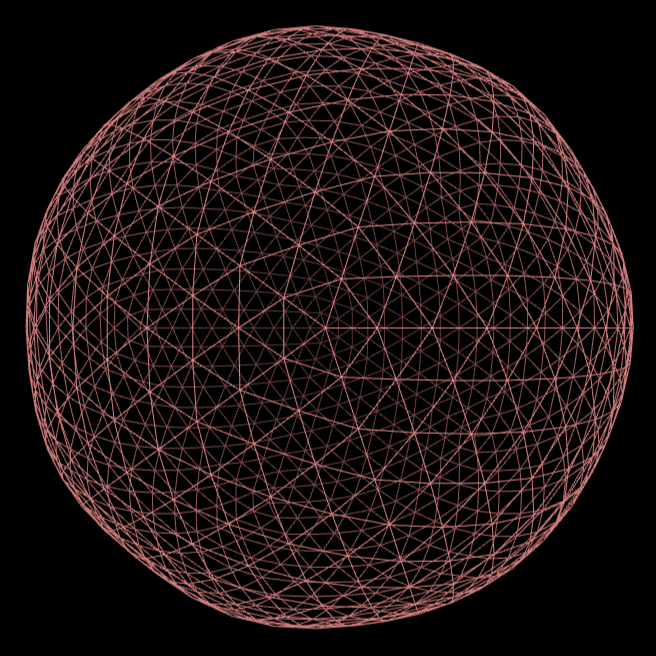
\includegraphics{1.png}
\begin{center}
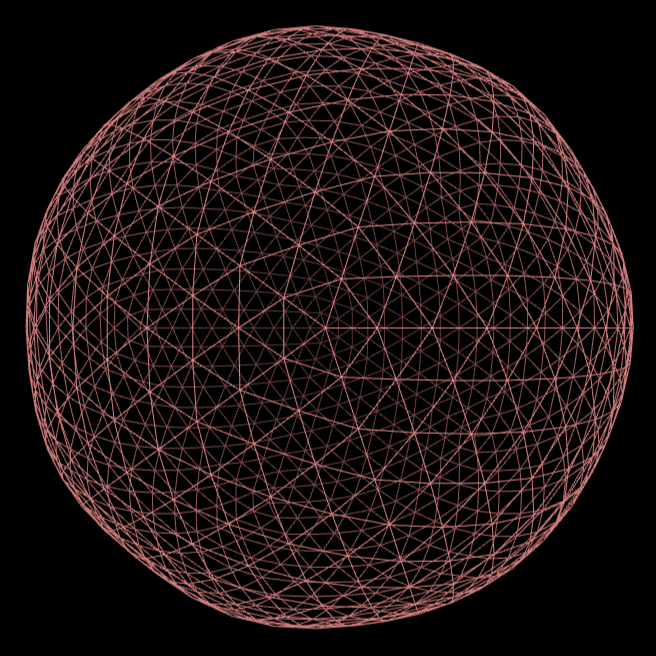
\includegraphics[width=9cm, height=9cm]{03.png}
\end{center}\\

\begin{center}
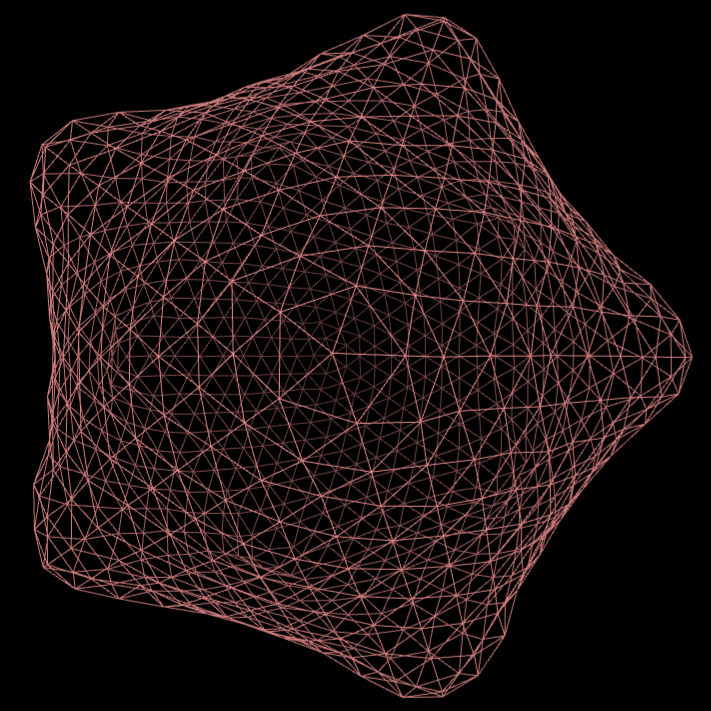
\includegraphics[width=9cm, height=9cm]{04.png}
\end{center}\\

\\
در قدم بعدی به شبیه غشا نانوذرات را نیز اضافه کردیم. در این مرحله علاوه بر تنظیم پارامتر های فبل باید واحد های مورد نیاز برهمکنش لنارد جونز را هم تنظیم کنیم.

در شکل زیر سایز نانوذره را در مقایسه با سایز غشا مشاهده میکنیم
در این شکل برهمکنشی بین غشا و نانوذره تعریف نشده و صرفا برای مقایسه ابعاد و یکسان بود ساختار غشا و نانوذرات نشان داده شده است.
\\.
\begin{center}
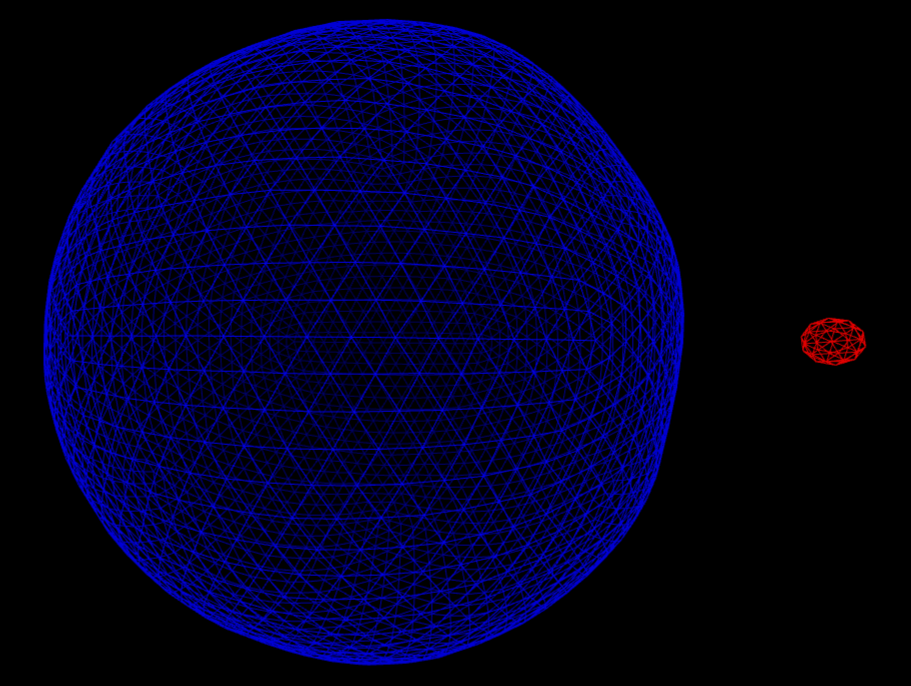
\includegraphics[width=11cm, height=9cm]{20210209_195305.png}
\end{center}\\

در ادامه برهمکنش غشا نانوذرات را   بررسی میکنیم
ابتدا یک نانو ذره را همراه غشا شبیه سازی میکنیم.
در این برهمکنش با توجه به اینکه از پتانسیل لنارد جونز استفاده شده و پارامتر های مهم این پتانسیل نیز عمق چاه و سیگما است \\
%نظیمن پارامتر ها  میتوان برهمکنش را مشاهده کرد%%% 
با تنظیم پارامتر های برهمکنش غشا با یک نانو ذره با توجه به عمق چاه پتانسیل لنارد جونز نانو ذره ابتدا درون غشا رها میشود و پس از آن به دیواره غشا میچسبد.
با توچه به شکل های نشان داده شده نانوذره ابتدا درون غشا و سپس به دیواره چسبیده است.
\begin{center}
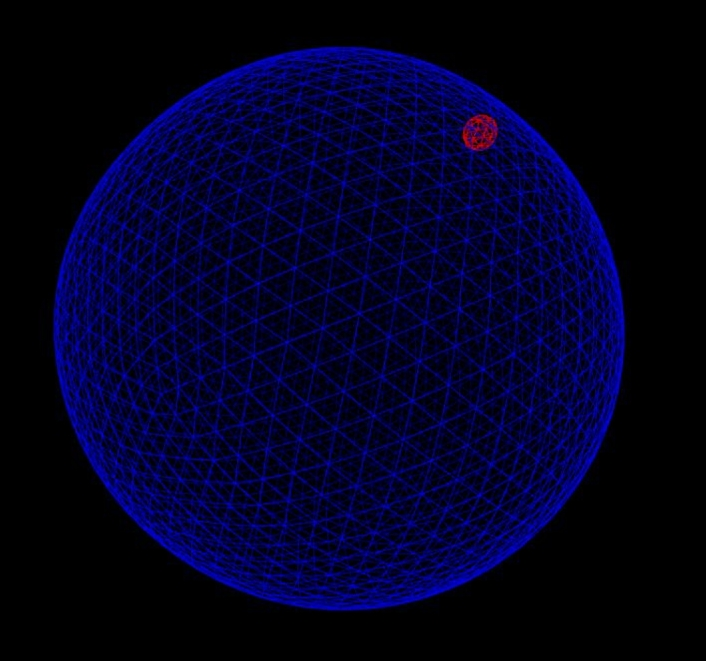
\includegraphics[width=9cm, height=9cm]{20210214_160511.jpg}
\end{center}\\
\begin{center}
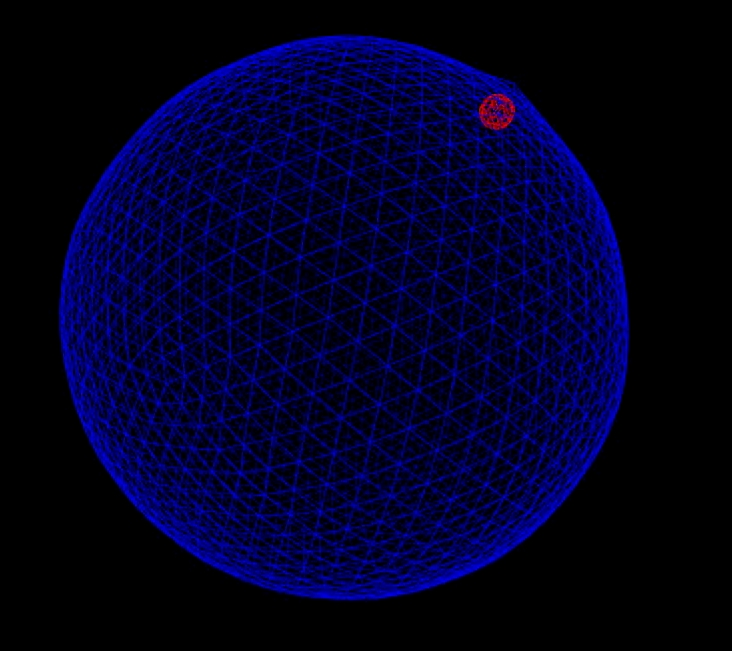
\includegraphics[width=9cm, height=9cm]{20210214_160439.jpg}
\end{center}\\

پس از مشاهده برهمکنش غشا و یک نانو ذره به سراغ مشاهده ی سیستم با دو نانو ذره میرویم.با افزایش قدرت پتانسیل برهمکنش مشاهده میکنیم که غشا به 
دور نانوذرات پیچیده شده است.
\begin{center}
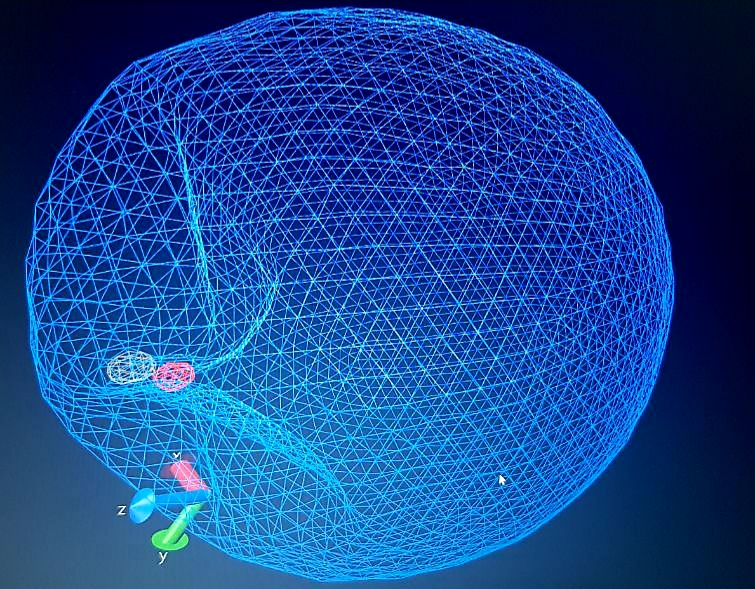
\includegraphics[width=11cm, height=9cm]{20210213_204324.jpg}
\end{center}\\




\begin{center}
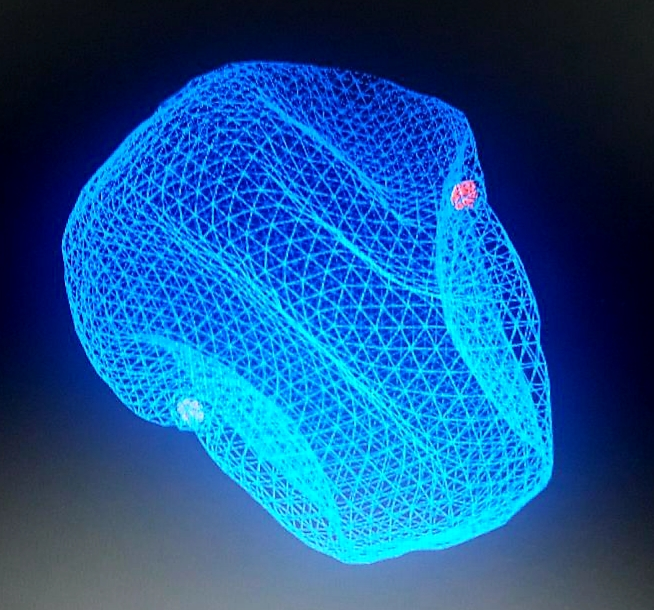
\includegraphics[width=11cm, height=9cm]{20210213_204232.jpg}
\end{center}\\


با توجه به نتایج شبیه سازی بسیار محتمل است که در برهمکنش غشا با دو نانوذره نانوذرات به یک دیگر نزدیک شوند . با توجه به اینکه هیچ نسرو جاذبه ای بین نانوذرات تعریف نشده ااین نزدیک شدن به علت به وجود آمدن نیروی موثری است که از برهمکنش همزمان غشا با نانوذره ایجاد میشود .در نتیجه غشا هزینه انرژی خمشی کمتری برای در بر گرفتن نانوذرات هزینه میکند.\\
در شکل های زیر مشاهده میکنیم که دو نانوذره به یک دیگر نزدیک شده اند.
شکل اول مکان اولیه نانوذرات را نشان میدهد.
شکل بعدی پس از 337 پیکو ثانیه شبیه سازی شده است.
\begin{center}
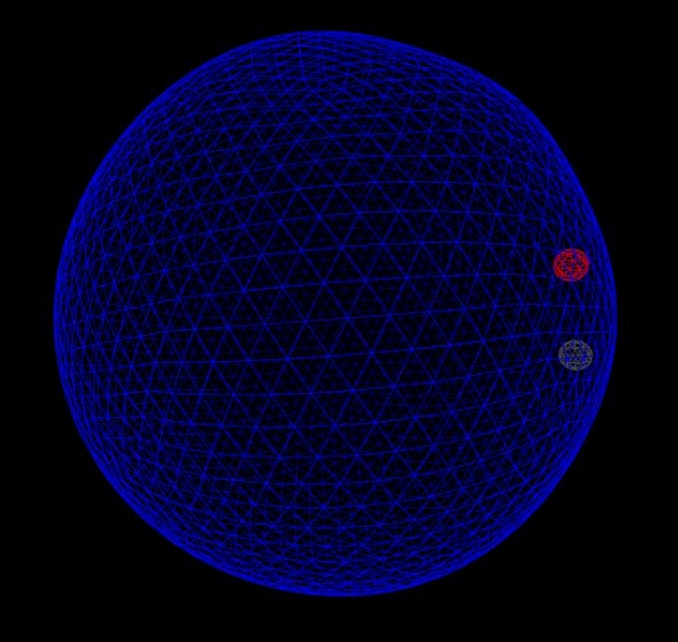
\includegraphics[width=9cm, height=9cm]{20210215_152251.jpg}
\end{center}\\

\begin{center}
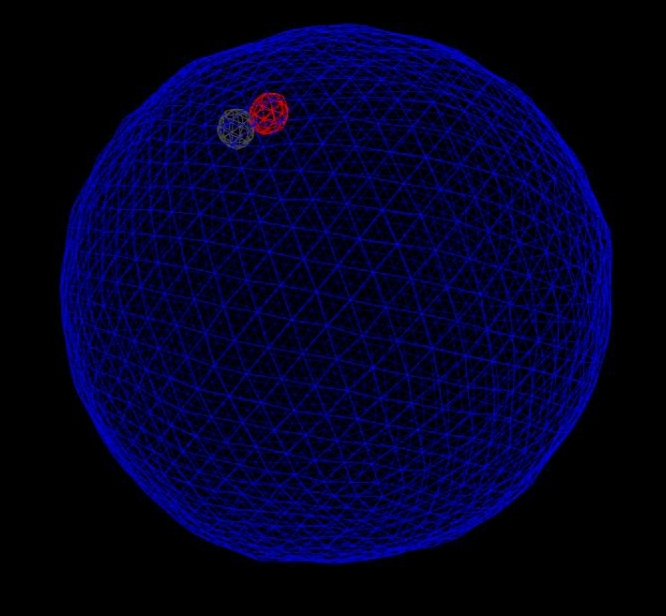
\includegraphics[width=9cm, height=9cm]{20210215_141728.jpg}
\end{center}\\




\section{\LARGE{جمع بندی}}
با توجه به نتایج شبیه سازی نشان داده شده دو نوع ساختار کلی غشا ی مایع و کشسان به وجود می آید. در برهمکنش غشا با ذرات غشا به عنوان یک واسطه موجب القای نیروی جاذبه میان نانوذرات میشود تا با صرف انرژی کمتر خمشی باعث کاهش انرژی کل سیستم شود.\\




\section{\LARGE{ارجاعات}}

%\bibitem{}
\lr{https://github.com/yeganeh1212/VCM-report/blob/main/config}\\
%20file.txt
%\bibitem{}
\lr{https://github.com/yeganeh1212/VCM-report/blob/main/FarsiThesis.pdf}\\
%\bibitem{}
\lr{https://github.com/yeganeh1212/VCM-report/blob/main/4_6046088568533682072.pdf}



%\end{thebibliography}









\end{document}